Integer programming expands upon the possible problems that can be modeled by
linear programming. Whereas decision variables in linear programming are
optimized on a continuum, i.e., all decision variables are real numbers,
$x \in \mathbb{R}^n$. Integer programming allows for decision variables to take
on integer-only values, i.e., $y \in \mathbb{Z}^n$. Strictly speaking, a
programming formulation for which all decision variables are integer (i.e.,
integer and binary) is called an \textit{integer program} (IP), whereas a
programming formulation for which some deicision variables are integer while
others are linear is called a \textit{mixed integer-linear program} (MILP). The
discussion that follows is informed largely by Wolsey's
text \cite{wolsey_integer_1998} from which I cite many definitions,
etc. Additional clarification comes from class notes \cite{luedtke_class_2010}.

Integer programming allows one to model specialized decision cases. Take for
example one of the most well-known problems in mathematical programming and
optimization, the \textit{Knapsack Problem}. The Knapsack problems is described
as follows:

\begin{itemize}
        \item A knapsack can hold at most $b$ pounds. 
        \item There are $n$ possible items that can be placed in the bag.
        \item Each item is characterized by a preference, or benefit, $c_i$, 
              and a weight, $a_i$
        \item One would like to maximize the benefit associated with a knapsack
\end{itemize}

The decision variables, $y_i$s, for the Knapsack Problem provide its integer
nature. Any given item in the above formulation can only be added once. Indeed,
consider that for any viable solution, each item is in one of two distinct
states: included in the knapsack or excluded from the knapsack. This duality of
states provides a natural usage of binary variables, i.e., a variable that has
only two states, 0 and 1. Accordingly, the Knapsack Problem as an integer
program is formulated as Equation \ref{eqs:knapsack}.

%%% 
\begin{subequations}\label{eqs:knapsack}
  \begin{align}
    %%
    \max \:\: & 
    \sum_{i \in I} c_i y_i
    & \\
    %%
    \text{s.t.} \:\: &
    \sum_{i \in I} a_i y_i \leq b 
    & \\
    %%
    &
    y_i \in \{ 0, 1 \}
    &
    \forall i \in I
    %%
  \end{align}
\end{subequations}
%%% 

\subsection{Computational Complexity}\label{sec:complexity}

In general, optimization problems are solved by solving a number of decision
problems. Decision problems are generally
computationally \textit{hard}. Decision problems ask yes or no questions,
e.g. ``is there a knapsack packing that with a benefit higher than $x$?''. An
optimization problem asks instead ``what is the knapsack packing with the
highest benefit?''. Any problem can be associated with one of four categories of
computational complexity:

\begin{itemize}
        \item Polynomial ($\mathcal{P}$)
        \item Nondeterministic Polynomial ($\mathcal{NP}$)
        \item Nondeterministic Polynomial Complete  ($\mathcal{NP}$-C)
        \item Nondeterministic Polynomial Hard  ($\mathcal{NP}$-hard)
\end{itemize}

The topic of computational complexity is relatively involved, thus I will only
provide a short overview to simply provide context. A problem is considered to
reside in $\mathcal{P}$ if there is a polynomial-time algorithm that can solve
it. A classic example is that of naive matrix inversion, known to be of order
$n^3$ (i.e., $\mathcal{O}(n^3)$) for a given $n$ x $n$ matrix.

A decision problem is considered to be in ($\mathcal{NP}$) if for any proposed
solution, there is a \textit{short certificate}.

\begin{define}
A \textbf{certificate} is a method to verify that a solutions provides a
positive or negative response to the question at hand. A certificate is
considered \textbf{short} if it is polynomial in size and can be verified in
polynomial time.
\end{define}

A decision problem, $Q$, is considered to be in $\mathcal{NP}$-C, if
$Q \in \mathcal{NP}$ and \textit{any} problem, $P \in \mathcal{NP}$ is
polynomially reducable to $Q$, i.e., instances of $P$ can be reformulated as
instances of $Q$ in polynomial time. The most popular candidate of this
polynomial reduction is the Satisfiabiliy Problem, known to be in
$\mathcal{NP}$-C.

Finally, a problem $Q$, is in $\mathcal{NP}$-hard, if any problem
$P \in \mathcal{NP}$ is polynomially reducible to $Q$, but
$Q \not\in \mathcal{NP}$. If a decision problem is in $\mathcal{NP}$-C, then the
corresponding optimization problem is $\mathcal{NP}$-hard.

The various levels of complexity are related. It is not known whether
$\mathcal{P} = \mathcal{NP}$, but it is strongly suspected that
$\mathcal{P} \subset \mathcal{NP}$. It is also assumed that
$\mathcal{NP}\text{-C} \subset \mathcal{NP}$, and
$\mathcal{NP}\text{-hard} \notin \mathcal{NP}$ by definition. The relationship
between these set of problem complexities is shown graphically in
Figure \ref{fig:complexity}.

\begin{figure}[H]
  \begin{center}
    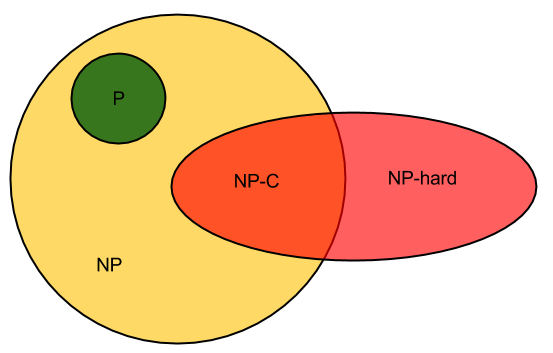
\includegraphics[width=\linewidth]{./chapters/litreview/complexity.png}
  \caption{The relationship between the various types of problem complexities.}
  \label{fig:complexity}
  \end{center}
\end{figure}


\subsection{Formulations and Cutting Planes}\label{sec:formulations}

Optimization problems are given as formulations, a series of inequality
equations. Both domain knowledge and geometrical investigation can provide
better formulations than may be evident from an initial formulation. Formally, a
formulation forms a polyhedron.

\begin{define}\label{def:polyhedron}
A subset of $\mathbb{R}^n$ described by a finite set of linear constraints $P
= \{ x \in \mathbb{R}^n : Ax \leq b\}$ is a \textbf{polyhedron}.
\end{define}

\begin{define}\label{def:formulation}
A polyhedron $P \subseteq \mathbb{R}^{n+p}$ is a \textbf{formulation} for a set
$X \subseteq \mathbb{Z}^n \times \mathbb{R}^p$ iff $X = P \cap \left( 
\mathbb{Z}^n \times \mathbb{R}^p \right)$
\end{define}

As previously noted, more than one formulation can be viable for a given
problem. Let us return to the Knapsack Problem in
Equation \ref{eqs:knapsack}. Consider a knapsack with $b = 5$ and items with
$a_1 = 2$, $a_2 = 3$, $a_3 = 4$. The original formulation is as follows.

%%% 
\begin{subequations}\label{eqs:knapsack1}
  \begin{align}
    %%
    \max \:\: & 
    \sum_{i \in I} c_i y_i
    & \\
    %%
    \text{s.t.} \:\: &
    2y_1 + 3y_2 + 4y_3 \leq 5 
    & \\
    %%
    &
    y_i \in \{ 0, 1 \}
    &
    \forall i \in I
    %%
  \end{align}
\end{subequations}
%%% 

The set of feasible solutions here forms a polyhedron from the points $Y = {(0,
0, 0), (1, 0, 0), (0, 1, 0), (0, 0, 1), (1, 1, 0)}$. The optimal solution will
depend on values given to each item's benefit, $c_i$. However, the formulation
as provided defines a solution space larger than the specific points mentioned
here. One could add a constraint, say, 

\begin{equation*}
y_1 + y_3 \leq 1
\end{equation*}

or 

\begin{equation*}
y_2 + y_3 \leq 1.
\end{equation*}

These two constraints state that the third item, if chosen, can not be included
with either the first or the second item. The resulting formulation is shown in
Equation \ref{eqs:knapsack2}.

%%% 
\begin{subequations}\label{eqs:knapsack2}
  \begin{align}
    %%
    \max \:\: & 
    \sum_{i \in I} c_i y_i
    & \\
    %%
    \text{s.t.} \:\: &
    2y_1 + 3y_2 + 4y_3 \leq 5 
    & \\
    %%
    &
    y_1 + y_3 \leq 1        
    & \\
    %%
    &
    y_2 + y_3 \leq 1        
    & \\
    %%
    &
    y_i \in \{ 0, 1 \}
    &
    \forall i \in I
    %%
  \end{align}
\end{subequations}
%%% 

It is obvious that Equation \ref{eqs:knapsack2} is a different formulation than
Equation \ref{eqs:knapsack1}. For example, the point $(0.9, 0.5, 0.4)$ resides
in the feasible solution space of Equation \ref{eqs:knapsack1} but is outside of
the feasible solution space of Equation \ref{eqs:knapsack2}. Intuitively, a
smaller solution space can be searched more quickly, thus \textit{tighter}
formulations require less time to solve in general.

The notion of one formulation being ``better'' than another can be formally
expressed.

\begin{define}
Given a set $X \subseteq \mathbb{R}^n$ and two formulations, $P_1$ and $P_2$,
for $X$, $P_1$ is a \textbf{better formulation} than $P_2$ if $P_1 \subset P_2$.
\end{define}

There is, of course, a limit to the formulations one can develop for a given
problem. A fully-restricted solution space, i.e., one that is as tightly bounded
as possible, is called the problem's \textit{convex hull}. 

\begin{define}
Given a set $X \subseteq \mathbb{R}^n$, the \textbf{convex hull} of $X$, denoted
$conv(X)$, is defined as: $conv(X) = \{x : x = \sum_{i=1}^{t} \lambda_i
x_i, \sum_{i=1}^{t} \lambda_i = 1, \lambda_i \geq 0$ for $i = 1, \ldots, t$ over
all finite subsets $\{x^1, \ldots, x^t \}$ of $X\}$.
\end{define}

Because the extreme points of $conv(X)$ all lie in $X$, the equivalent LP can be
used instead of the IP. Convex hull formulations are rarely seen in practice,
however, because they require an exponential number of additional
constraints \cite{wolsey_integer_1998}. While the convex hull of a given problem
may not be discovered in practice, the feasible solution space most assuredly is
reduced by most solution techniques. From a geometrical point of view, this acts
as cutting off solution space from some original larger space through the
addition of constraints as shown above. Accordingly, these additional
constraints are termed \textit{cutting planes}.

\subsection{The Branch and Bound Algorithm}\label{sec:bnb}

One of the most popular solution techniques used to solve integer programs is an
algorithm called \textit{Branch and Bound} (BNB). At its core, BNB is a divide
and conquer search algorithm that uses an enumeration tree to find optimal
solutions to $\mathcal{NP}$-hard IPs and MILPs. There are a number of ways to
speed up the search based on general techniques and problem-specific insights, a
number of which have been discussed in the previous section. In this section,
I'd like to highlight the basic nature of the algorithm and discuss lightly some
of the variety of solution strategies available. Again, the discussion here
comes largely from \cite{wolsey_integer_1998} and \cite{luedtke_class_2010}.

BNB utilizes the \textit{relaxation} of a given IP or MILP. A relaxation is a
related reformulation of a given problem that is generally easier to solve. In
the case of a linear programming relaxation, integer variables in the IP or MILP
are relaxed and allowed to be linear variables. Solving this formulation is
advantageous because it provides an \textit{upper bound} for the IP or
MILP. Similarly, solving a dual, given that it is feasible and has a finite
solution, or using some other heuristic provides a \textit{lower bound}. These
bounds allow the search tree to terminate, or \textit{prune}, a
given \textit{branch}.

A simple example greatly helps to show the process of the BNB algorithm. Let us
use a specific instance of Equation \ref{eqs:knapsack}. This example is
contritite and does not involve pruning; it is useful simply to show how
branching occurs. Consider a knapsack with three items. The items have benefits
of 0.5, 1, and 1.4, respectively and weights of 2, 3, and 4 pounds,
respectively. The knapsack can hold 5 pounds. The integer program is shown in
Equation \ref{eqs:knapsack-ip} and the LP relaxation is shown in
Equation \ref{eqs:knapsack-lp}.

%%% 
\begin{subequations}\label{eqs:knapsack-ip}
  \begin{align}
    %%
    \max \:\: & 
    Z^{IP} = 0.5 y_1 + y_2 + 1.4 y_3
    & \\
    %%
    \text{s.t.} \:\: &
    2y_1 + 3y_2 + 4y_3 \leq 5 
    & \\
    %%
    &
    y_1, y_2, y_3 \in \{ 0, 1 \}
    %%
  \end{align}
\end{subequations}
%%% 

%%% 
\begin{subequations}\label{eqs:knapsack-lp}
  \begin{align}
    %%
    \max \:\: & 
    Z^{LP} = 0.5 y_1 + y_2 + 1.4 y_3
    & \\
    %%
    \text{s.t.} \:\: &
    2y_1 + 3y_2 + 4y_3 \leq 5 
    & \\
    %%
    &
    y_1, y_2, y_3 \in [0, 1]
    %%
  \end{align}
\end{subequations}
%%% 

Solving the relaxation provides an upper bound of $Z^{LP} = \frac{26}{15}$, a
(non-integer) solution of $y' = (0, \frac{1}{3}, 1)$ and a root node for the BNB
search tree, shown in Figure \ref{fig:root}.

\begin{figure}[H]
  \begin{center}
    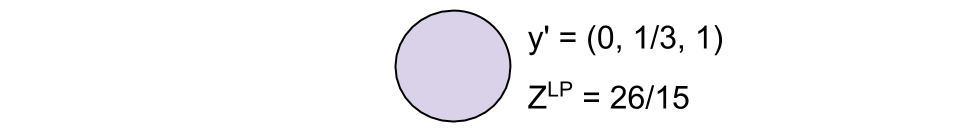
\includegraphics[width=\linewidth]{./chapters/litreview/root.png}
  \caption{The root node for the BNB algorithm associated with 
  Equation \ref{eqs:knapsack-ip}.}
  \label{fig:root}
  \end{center}
\end{figure}

The algorithm then chooses a variable on which to \textit{branch}. Formally
branching divides the set of feasible solution spaces in two. Given a solution
space $S$, branching on a binary variable $y_i$, produces two new solution
spaces.

\begin{equation}
\begin{split}
& S_1 = S \cap \{y: y_i = 0\}
\\
& S_2 = S \cap \{y: y_i = 1\}
\end{split}
\end{equation}

If the variable is non-binary integer, given a non-integer feasible solution,
$y'$, one produces the following new spaces.

\begin{equation}
\begin{split}
& S_1 = S \cap \{y: y_i \leq \lfloor y_i' \rfloor\}
\\
& S_2 = S \cap \{y: y_i \geq \lceil y_i' \rceil\}
\end{split}
\end{equation}

Arbitrarily, for this example case, one could choose to branch on
$y_2$. The resulting relaxations are shown as Equation \ref{eqs:y2-0} for $y_2 =
0$ and Equation \ref{eqs:y2-1} for $y_2 = 1$.

%%% 
\begin{subequations}\label{eqs:y2-0}
  \begin{align}
    %%
    \max \:\: & 
    Z^{LP} = 0.5 y_1 + 1.4 y_3
    & \\
    %%
    \text{s.t.} \:\: &
    2 y_1 + 4 y_3 \leq 5 
    & \\
    %%
    &
    y_1, y_3 \in [0, 1]
    %%
  \end{align}
\end{subequations}
%%% 

%%% 
\begin{subequations}\label{eqs:y2-1}
  \begin{align}
    %%
    \max \:\: & 
    Z^{LP} = 0.5 y_1 + 1 + 1.4 y_3
    & \\
    %%
    \text{s.t.} \:\: &
    2 y_1 + 3 + 4 y_3 \leq 5 
    & \\
    %%
    &
    y_1, y_3 \in [0, 1]
    %%
  \end{align}
\end{subequations}
%%% 

Each of these new subproblems become \textit{active nodes} and are added to
the \textit{active list}. Active nodes are subproblem nodes that have been
recognized by the algorithm and the next subproblem to solve is chosen from the
active list by some strategy. For this simple case, both subproblems are solved
and the resulting values are shown in Figure \ref{fig:branch}.

\begin{figure}[H]
  \begin{center}
    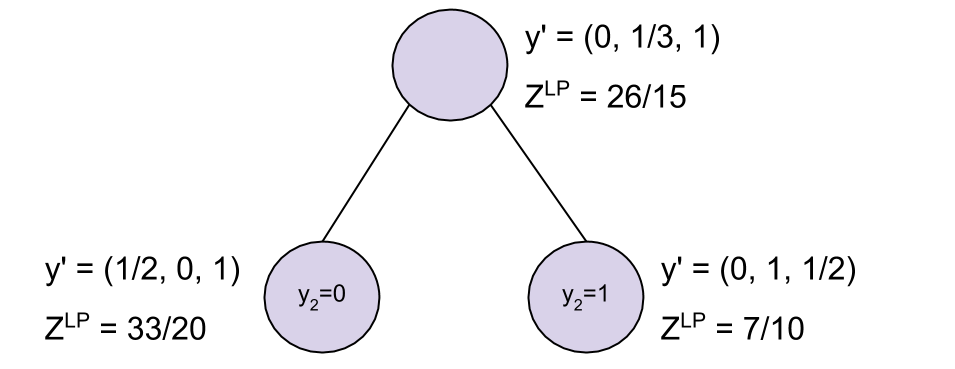
\includegraphics[width=\linewidth]{./chapters/litreview/branch.png}
  \caption{The first two branches of the BNB algorithm associated with 
  Equations \ref{eqs:y2-0} and \ref{eqs:y2-1}.}
  \label{fig:branch}
  \end{center}
\end{figure}

One could continue in this manner, branching on subsequent variables and
enumerating all possible solutions, to eventually reach the optimal solution of
$y^* = (1, 1, 0)$. However, so far we have ignored pruning, the act of
terminating a branch of the search tree, knowing that no further useful
information can be gained from its investigation. Pruning provides the
``bounding'' aspect of the Branch and Bound algorithm.

At any point in the process of the BNB algorithm, there is a known global upper
bound, $U$, to the optimal solution and lower bound, $L$, to the optimal
solution. Accordingly, a branch of the enumeration search tree can be pruned in
three instances:

\begin{enumerate}
        \item The subproblem is optimal, given its subspace of the feasible
        option space.
        \item The subproblem has a known upper bound that is lower
        than the global lower bound or the subproblem has a known lower bound
        that is larger than the global upper bound.
        \item The subproblem is infeasible.
\end{enumerate}

With the above background, the actual BNB algorithm can be presented.
\\
\begin{algorithm}[H]
 \SetAlgoLined
 \KwData{Decision variables, an objective function, and a set of constraints.}
 \KwResult{Optimal values for the decision variables or a flag denoting 
   infeasibility or unboundedness.}
 Perform any \emph{preprocessing operations}\;
 Derive a lower bound, $L$, via a \emph{heuristic}\;
 Place original problem on the active list\;
 \While{The active list is \textit{not} empty}{
       Use a \emph{strategy} to select a candidate node ($S$) from the active 
       list\;
       Solve the LP relaxation to get an upper bound for the candidate, $U(S)$\;
       \If{$U(S) > U$}{$U \leftarrow U(S)$\;}
       \If{$S$ is infeasible}{
           prune the branch\;
       }
       \ElseIf{$U(S) > L$}{
           $L \leftarrow U(S)$\;
       }
       \ElseIf{$U(S) < L$}{
           prune the branch\;
       }
       \Else{
           branch on $S$\;
           add new subproblems to the active list\;
       }           
       Remove $S$ from the active list\;
 }
 \caption{The Branch and Bound Algorithm}
\end{algorithm}

There are three ways to assist, or speed up, the Branch and Bound algorithm as
highlighted above:
\begin{enumerate}
        \item Preprocessing
        \item Lower-bound heuristics
        \item Node selection strategies
\end{enumerate}

Preprocessing is a step provided by many solvers. It generally involves an
investigation of the problem instance in order to minimize future
work. Preprocessing can affect solution bounds by tightening bounds or providing
cutoffs to the solver (i.e., preformed feasible solutions). It can speed up the
internal Simplex Method processing by informing the solver as to good simplex
pricing strategies. The feasible solution space can also be reduced by finding
redundant constraints and providing cutting planes, as discussed in the previous
section. Finally, the preprocessing step can \textit{a priori} fix certain
decision variables. The variable fixing algorithm is straightforward.

\begin{algorithm}[H]
 \SetAlgoLined
 \KwData{An constraint matrix, $A$, objective coefficients, $c$, and decision 
 variables $x$ with decision variable lower bounds, $l$, and upper bounds 
 $u$.}
 \KwResult{A (possibly empty) set of fixed variables.}
 \ForEach{decision variable, $x_j$,}{
   \If{$a_{i,j} \geq 0 \;\; \forall \;\; i$ {\emph{and}} $c_j < 0$}{
     $x_j \leftarrow l_j$\;
   }
   \ElseIf{$a_{i,j} \leq 0 \;\; \forall \;\; i$ {\emph{and}} $c_j > 0$}{
     $x_j \leftarrow u_j$\;
   }       
 }  
 \caption{The Variable Fixing Algorithm for a Maximization Objective Function}
\end{algorithm}

A variety of lower-bound heuristics exist. Some of the most popular involve
solving heavily restricted versions of the original problem or diving down the
enumeration tree, rounding fractional integer values. There are also
problem-specific heuristics that depend on well-known problem structures.

Finally, there exist nominally three well-used node selection strategies. The
first is called the \textit{Best Node Search} (BNS) which chooses the next best
node in the active list based based on the node's upper bound. This requires
large movement around the search tree, effectively solving dissimilar
relaxations. The second is the well-known \textit{Depth First Search} (DFS). A
DFS for an IP-enumeration tree is beneficial because subsequent relaxations are
related, which allows for \textit{warm start} of the LP relaxations. Warm starts
allow subsequent relaxations to be solved quickly because good approximations to
the optimal solution can be provided. The final strategy is a \textit{BNS-DFS
hybrid}. The hybrid strategy involves estimating an optimal value, performing a
DFS until the relaxation's optimal value is below that of the estimation, and
then choosing the next-best node to continue.
